\documentclass[10pt]{article}
\usepackage{graphicx}
\usepackage{subcaption}
\usepackage[T1]{fontenc}
\usepackage{amsmath}
\usepackage{lipsum}
\usepackage{amsfonts}
\usepackage{hyperref}
\usepackage{mathtools}
\providecommand\given{}
\usepackage[utf8]{inputenc}
\usepackage[letterpaper,margin=1in]{geometry}
\usepackage[parfill]{parskip}

\def\therefore{\boldsymbol{\text{ }
\leavevmode
\lower0.4ex\hbox{$\cdot$}
\kern-.5em\raise0.7ex\hbox{$\cdot$}
\kern-0.55em\lower0.4ex\hbox{$\cdot$}
\thinspace\text{ }}}

\vspace{-8ex}
\date{}

\graphicspath{ {./figs/} }

\begin{document}

\title{\textbf{\Large{\textsc{ECE410:} Linear Control Systems}} \\ \Large{Lab 1 Report: NL Sims?} \\ \textbf{\small{PRA101}}\vspace{-0.3cm}}
\author{Pranshu Malik, Varun Sampat \\ \footnotesize{1004138916}, \footnotesize{1003859602}\vspace{-3cm}}

\maketitle

\section{Introduction}
We have a system $G(s)$ that is very nice.

\begin{figure}[h]
 \centering
 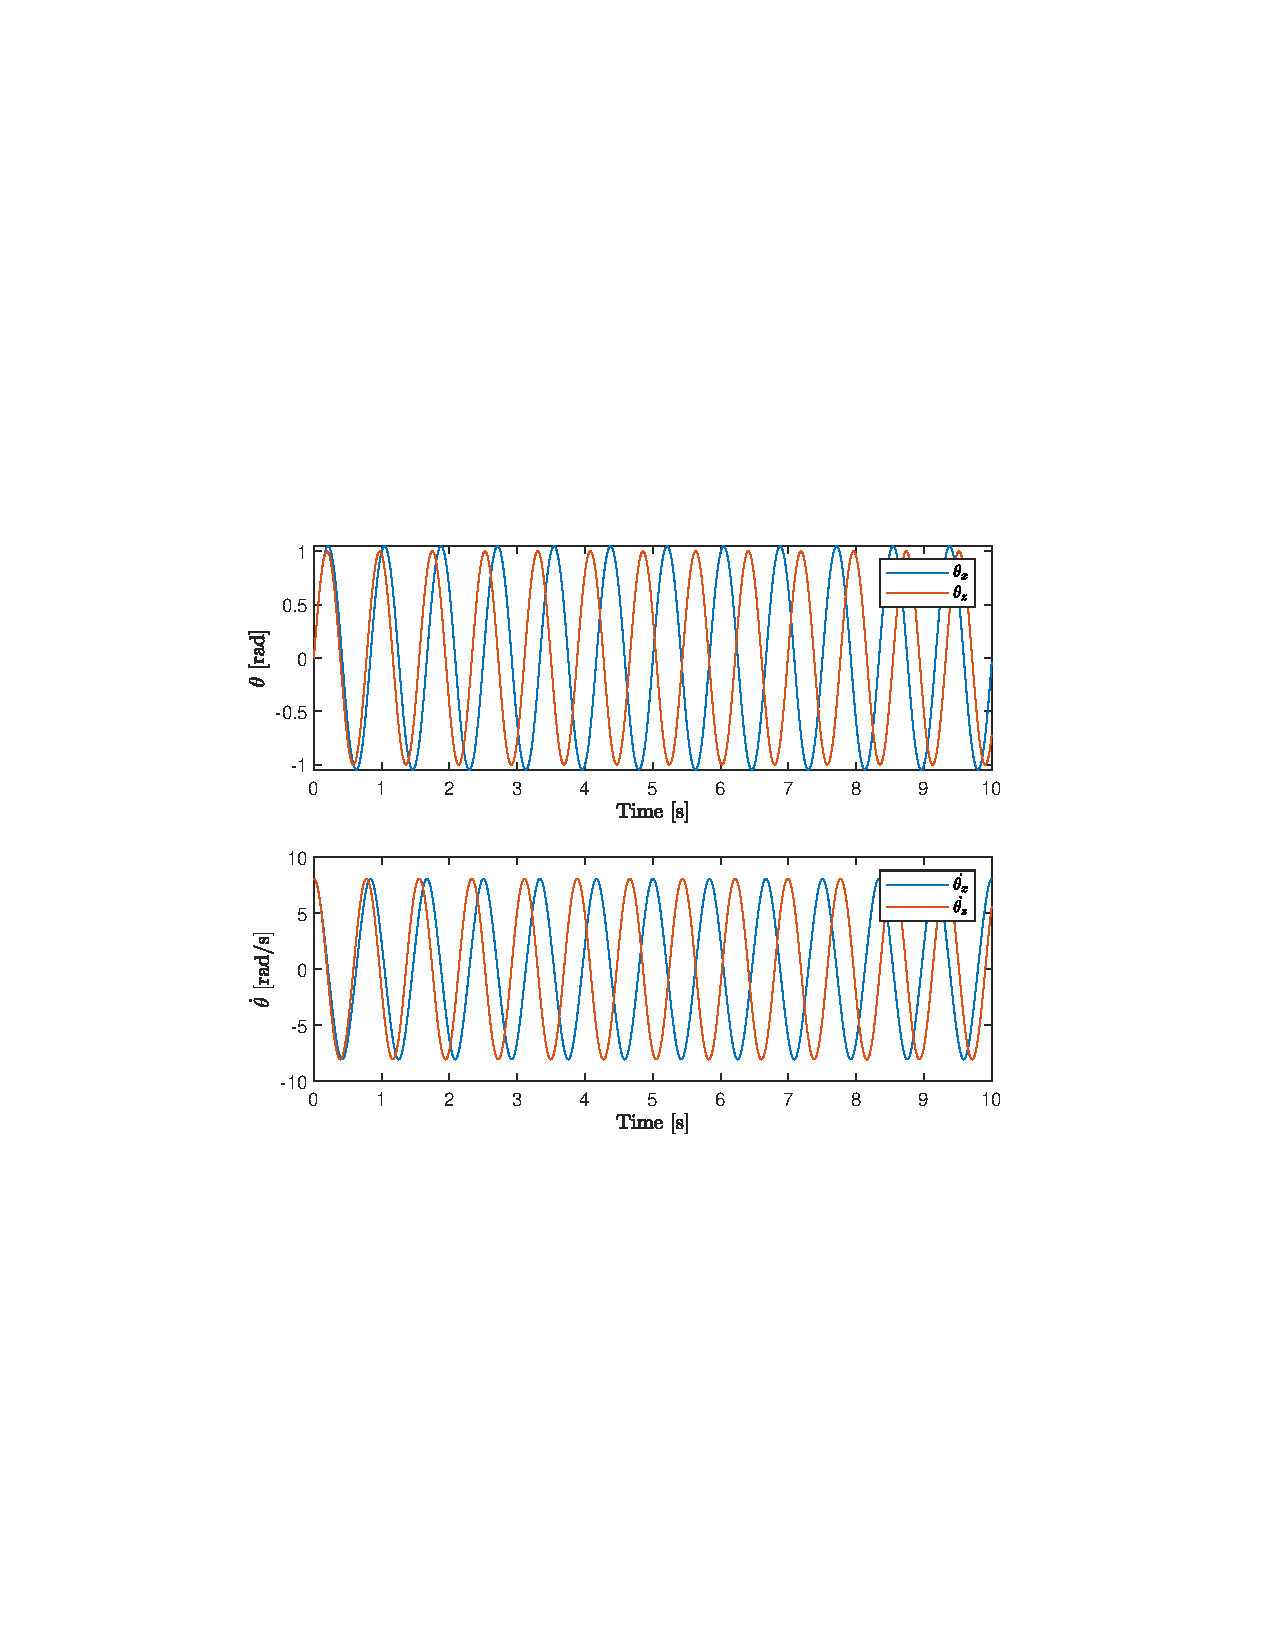
\includegraphics[clip, scale=0.7, trim=0.5cm 11cm 0.5cm 11cm, width=1.00\textwidth]{X_0_1_state_evolution.pdf}
 \caption{test123}
 \label{figure:test123}
\end{figure}

Figure out trimming this way:
\newpage
\fbox{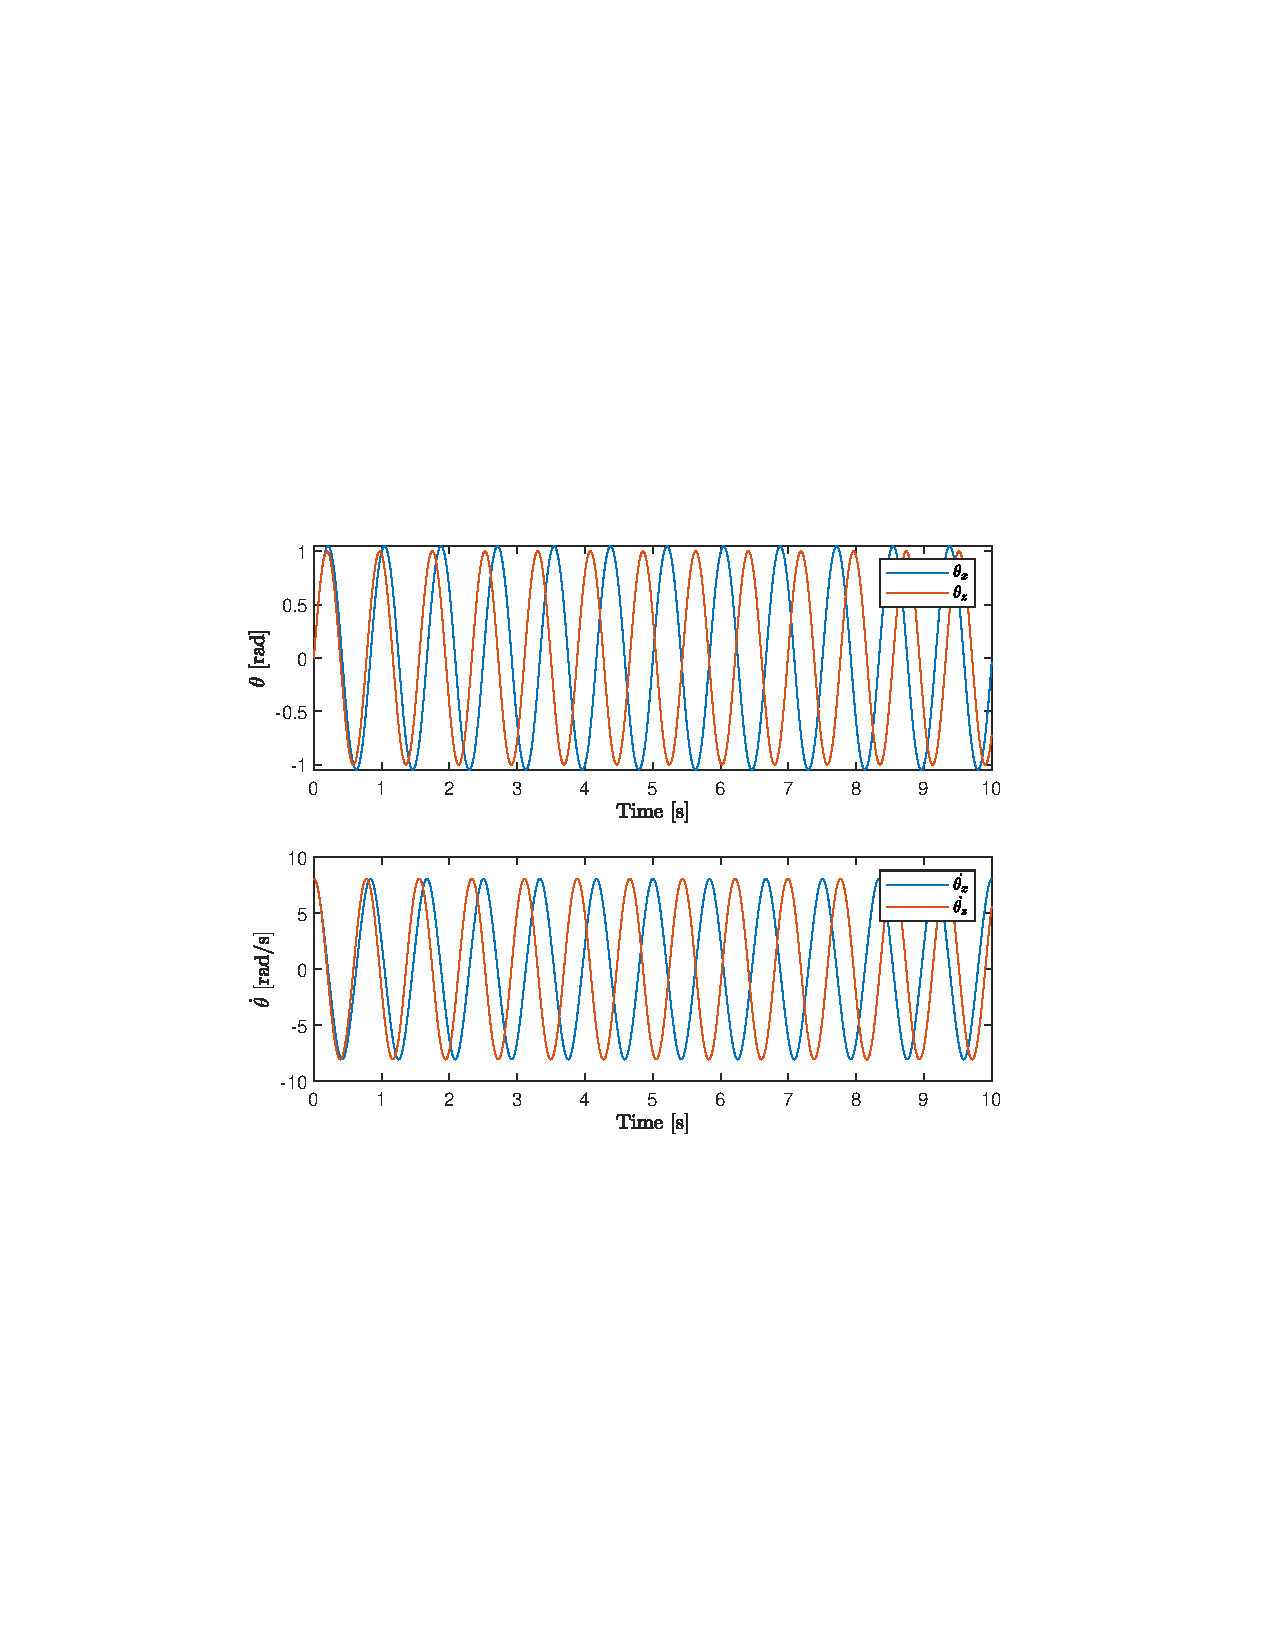
\includegraphics[scale=0.7, trim=0.5cm 11cm 0.5cm 11cm]{X_0_1_state_evolution.pdf}}

Test123



\end{document}
